\documentclass[11pt]{article}   % or report, book, beamer (slides)

% --- Preamble ---
\usepackage{amsmath, amssymb, amsthm}  % math essentials
\usepackage{graphicx}                  % images
\usepackage{booktabs}                  % table rules
\usepackage{hyperref}                  % clickable links/refs (load near last)
\usepackage[backend=biber, style=authoryear]{biblatex}
\usepackage[margin=1in]{geometry} 

\addbibresource{references.bib}
\title{Bluesky Case Study Report}
\author{Gabriel Burr}
\date{\today}

% --- Body ---
\begin{document}
\maketitle

\section{Abstract}
The effect of online echo chambers on political polarization is a contentious topic in contemporary media studies and political science \parencite{Cinelli2021}.
With a potential panoply of negative effects—from individual real-world hate crimes to an erosion of the American democratic system—the topic poses an urgent issue that empirical studies have nonetheless remained divided on in recommendation. The two predominant theories on the topic are the
contact hypothesis \parencite{Allport1979}, which argues an exposure to alterity grounded in sameness reduces hostility, and a reactionary theory instead predicting backfire effects \parencite{Bail2018}. 
Both sides have conducted studies finding evidence in favor of their positions, and so the question of policy is at an impasse. We contend that these muddled findings are themselves indicative 
of a more structural flaw in modern communication, propose that Baudrillard can supply the vocabulary to describe it with his concept of a ``hell of the Same,'' 
and analyze a Bluesky database to attempt to find evidence for an operationalized version of it by sorting individuals into communities and measuring in-group responses of similar posts by both in and out-group authors.

\section{Introduction}\label{sec:introduction}
The general consensus regarding this topic is that platforms and policymakers should aim to reduce online hostility as such. This assumes, 
however, that the actual harms associated with online polarization are reliably tracked by online hostility itself. Following Baudrillard, we instead posit that the digital 
Other encountered on these platforms  cannot present as the genuine alterity required for embodied symbolic exchange, and so is consumed as a sign of difference that 
only propagates a binary worldview further rather than challenging it.

\subsection{A Hell of the Same}\label{sec:hell-of-the-same}
Baudrillard coins the phrase ``hell of the Same'' to describe the self-perpetuated expansion of this binary code \parencite{Baudrillard_1993}. Simply put, the code is the set of categories we use to
define ``me'' and ``not me.'' The danger is that with an increase in explanations we strip doubt from reality and reduce the foreign to the simply different, an object of
knowledge that can be understood rather than that which is truly Other. Physicality constrains one's subjectivity in embodied reality, but on social media profiles, slogans,
and trends offer up prepackaged meaning that allow us to readily domesticate the uncomfortable. For instance, a pro-Israeli user might share the same opinions on taxation
as a visibly pro-Palestinian profile, yet respond negatively to their expressed opinion on the topic despite substantive agreement; in that moment neither the Self nor the Other
matter, only the code of pro-Israel and anti-Israel.

\subsection{Significance}\label{sec:significance}
Let us focus on the two harms raised in the introduction:
real-world hate crimes and democratic erosion. Baudrillard identifies racism to be rooted in Enlightenment ideals of universal humanity, where it is this very universalization that permits us to
understand the Other and bring them into our world under labels like ``ill,'' ``insane,'' or ``primitive'' where they act as signs of difference which confirm our vitality, sanity, and advancement \parencite[pg. 129]{Baudrillard_1993}. An ontology
of difference is the foundation of not just hate crimes, but racism overall, so measures that aim to just reduce hostility while furthering this system defeat themselves at the outset. \bigskip

In a study performed by Balietti et al.\parencite*{Balietti2021}, participants on social media were surveyed and matched with like-minded peers, who then viewed their matched partner's profile before reading
a short essay written by them concerning wealth redistribution. The study then finds evidence for affective polarization decreasing when strong stance users matched with similar, opposing stance users, and
opposite effects for pairings of similar, same side users. Further, they found evidence that degree of sameness tracks degree of shift in stance. The authors take this conclusion to recommend community bridging
to reduce extreme opinions. \bigskip

It could also be argued, however, that the findings of this study were of participants who were willing to shift their views on a topic that should concern their livelihoods based on fidelity to role identity determined by an arbitrary algorithm.
They only ever encountered a simulacrum of the Other, so while affective polarization might empirically have decreased, it is evident that the binary code of ``me'' or ``not me'' has only been sharpened further: participants
have discovered that ``me'' holds a slightly more moderate view, since this Other who sits on my side of the difference holds a contrary opinion. This raises the question of what happens when someone sitting
on the other side of that difference is encountered, when one encounters—in a decidedly untailored embodied reality—a truly different Other who is more than an image of the Same.

\subsection{Application}\label{sec:application}
This is not to say that bridging is worthless, only that we should exercise more caution about when to recommend a community be exposed to more out-group content. A measure which seeks to
reduce bigotry but only provides a community with more signs to consume as fuel would fail or backfire, consistent with findings by Bail et al.\parencite*{Bail2018}. Instead, we propose testing the degree to which a community is receptive to content over role
before implementing policy measures, and use Bluesky as a case study example. If reception follows the sign regardless of content, bridging would be inadvisable. If instead exposure is the main determinant of out-group reception, then whatever recommendation algorithms that govern exposure are the right instrument for policy; feeds and 
follow recommendations should surface out-group authors in proportion to the relevance of their content rather than the size of their existing audience.

\subsection{Training Data}\label{sec:training}
It should be observed that recommendation algorithms are first-order cybernetic systems trained on the same engagement they shape.
Feeds consume interaction data in reposts, replies, and follows, and pull patterns from it to recommend content to users. This is where our empirical findings enter: an algorithm
trained on engagement alone would see in-group posts receiving 76\% of reposts (Section~\ref{sec:results}), when in fact this share mostly just reflects the author's audience itself
(Figure~\ref{fig:exposure-gap}). The model learns to route more exposure to already visible in-group authors and thus creates a feedback loop standardizing what users see. This manufactures
a hallucinatory in-group bias unrepresentative of the actual user's attitudes, and this is what our exposure-adjusted analysis seeks to address.

\section{Methodology}\label{sec:methodology}
Drawing upon a public database of 4M Bluesky users and 235M posts \parencite{FaillaRossetti2024, FaillaRossetti2025}, we pull a list of followers, a list of interactions, and the total corpus of posts. We then
create an undirected weighted edge graph using the followers list for edges and the interactions list for weights. Weights are handled evenly and summed, so a reply, a repost, and a quote count the
same for engagement. Notably, this only accounts for active users (users that have at least one interaction), dropping the number of handled accounts to 1.66M.

\subsection{Community Detection}\label{sec:communities}
We partition the active graph with the Leiden algorithm \parencite{Traag2019} to find users' ideological clusters, optimizing with regards to weighted modularity; i.e.
the portion of interaction weight that falls within a community beyond what might be expected from the user's aggregate activity.
In our implementation the algorithm yielded 24,802 communities with modularity $Q = 0.718$ on a set random seed. Running the model on different random seeds
showed that partitions were highly stable: pairwise NMI ranged from 0.875 to 0.95 on the full graph, taking a
sample of the top 100k most active users increased that to $\geq 0.99$.

\subsection{Content Embedding}\label{sec:embedding}
Each post was encoded with the sentence-transformer \texttt{all-mpnet-base-v2} \parencite{Reimers2019} and its nearest 20
neighbors were retrieved with an approximate HNSW index \parencite{Malkov2020} in FAISS
\parencite{Johnson2021}, where pairs by different authors were kept with cosine similarity $\geq 0.80$. We dropped any posts that would have a length of zero ignoring URLs
and mentions, and the threshold value was chosen after previewing a strata of random sample choices from 0.75 to 0.95. Since embedding similarity is insufficient to examine reception,
we next label stance separately (Section~\ref{sec:stance}), and only match pairs when both content and stance align for the primary analysis (pairs with same content and different stance are also kept as a robustness check.

\subsection{Stance Labelling}\label{sec:stance}

Stance labelling was done by a small LLM \parencite[following][]{QuelleBovet2025}, in our implementation
\texttt{claude-haiku-5-5} on low effort. For analysis we collapsed our stances into 3 (PAL, ISR, and other), but at this stage a codebook was drawn up with 7 available stances:
pro-Palestinian, pro-Israeli, anti-war humanitarian, critical of both, neutral news, unclear, and unrelated, with confidence levels from 1 to 3. The codebook was tuned on 200 posts hand annotated by the author, mainly to minimize the rate
of stance switches where sarcastic pro-Palestinian posts were falsely labelled as pro-Israeli. The codebook was then promptly frozen and ran against a separate test set of another 198 posts also hand annotated by the author (Table~\ref{tab:stance-accuracy}).
Label accuracy on the test set was moderate (65\%, $\kappa = 0.54$) in regards to the codebook labels, but side level accuracy fared much better at 76\%, important since that's what we actually used. Additionally, pro-Palestinian posts
switched sides only 1\% of the time, so our precision was similarly unimpacted. It's important to note that the rate of incorrect labels
was much higher for pro-Israeli posts (around a quarter in testing), so ISR labels are treated as exploratory. A total of 245,891 posts were labelled—having been slimmed down both by the embedding similarity threshold (Section~\ref{sec:embedding}) as well
as an initial regex query for posts involving the IS/PL conflict—and yielded in total 1.24M matched pairs, including 430,038 PAL-PAL, 58,298 ISR-ISR and 94,532 PAL-ISR.\bigskip

\begin{table}[h]
\centering
\begin{tabular}{lccc}
\toprule
 & Accuracy & Cohen's $\kappa$ & Side-level accuracy \\
\midrule
Dev (200 posts, tuned on) & 84\% & 0.79 & 90\% \\
\textbf{Test (198 posts, held out)} & \textbf{65\%} (95\% CI 59--72\%) & 0.54 & 76\% \\
\bottomrule
\end{tabular}
\caption{Agreement between the frozen Haiku labeller and the author's hand labels. Accuracy and $\kappa$ are over
the seven codebook labels; the side-level column collapses them to PAL, ISR and other.}
\label{tab:stance-accuracy}
\end{table}


\subsection{Contrasts}\label{sec:contrasts}
Since any in-group is always relative to some community, matched pairs are not themselves a sufficient measure of in-group reception. 
Our unit of analysis is instead the contrast; that is, a matched pair viewed from a single community $C$ to which exactly one of the two authors is beholden. That author's post is thus the
in-group post and the other is attributed to the out-group. Engagement with both posts is counted only from members of $C$ excluding self-engagement; further reposts are the
primary outcome here while replies, quotes and negative-tone replies are secondary measures, and we account for each author's exposure measured by their follower count in $C$. Since we determine that the two
posts in a contrast share content, stance and audience, a difference in how $C$ divides its engagement between them can be attributed to the author themselves over messaging (again, we control for exposure).

\subsection{Modeling}\label{sec:modeling}
Our unit of analysis is a contrast $r$ (Section~\ref{sec:contrasts}), which is a content pair seen from one community $C$. 
It has an in-group post $i$ and an out-group post $o$. We define the following for our model:

\begin{itemize}
    \item $y_{rp}$, which is engagement with post $p$ from members of $C$
    \item $F^{C}_p$, which tracks the author's followers who are in $C$ (controlling for exposure effects)
    \item $F^{\text{all}}_p$, which is the author's followers overall (also controlling for exposure more generally)
    \item $a_p$, which is the post's age
    \item $\Delta_r x = x_i - x_o$, which is the in-group minus out-group difference for any quantity $x$ within contrast $r$
\end{itemize}

Conditioning on each contrast's total engagement from $C$ within a pair is equivalent to a Poisson model with a fixed effect for each contrast, and it gives:
\[
y_{ri} \mid n_r \sim \operatorname{Binomial}(n_r,\ \pi_r), \qquad
\operatorname{logit} \pi_r = \beta + \gamma\, \Delta_r \log\!\left(1 + F^{C}\right)
  + \delta\, \Delta_r \log\!\left(1 + F^{\text{all}}\right) + \lambda\, \Delta_r a
\]

\subsubsection*{Quantity of interest}
The quantity of interest is the rate ratio $\text{RR} = e^{\beta}$. This is just $p_i$'s expected
engagement from $C$ relative to $p_o$'s (holding all other factors constant). $e^{\beta}$ is reported with a 95\% confidence interval, and
any CI that includes 1 implies no detectable difference. RR = 1 means no difference, and RR = 1.5 corresponds to a 60\% share. Standard errors are clustered both by in and out-group author since authors may reappear
in any number of contrasts. The primary sample is PAL-PAL contrasts in communities with at least 100 contrasts. Large communities with at least 1,000 contrasts are also reported individually. \bigskip

\subsubsection*{Robustness checks}
The following is also reported to verify the validity of the results:
\begin{enumerate}
    \item Keep only contrasts whose authors' followers in $C$ differ by less than a
    factor of $e$, i.e.\ $\left|\Delta_r \log(1 + F^{C})\right| \le 1$ (exposure-matching).
    \item The results of the PAL-ISR contrasts with similar content and opposite stances. 
    \item Keep only stance labels at confidence $\geq 2$ (Section~\ref{sec:stance}).
    \item Drop short, near-duplicate and linked pairs.
    \item The results of the exploratory ISR-ISR contrasts (Section~\ref{sec:stance}).

\end{enumerate}

\section{Results}\label{sec:results}
The 1,239,952 matched pairs yielded 1,437,993 contrasts, of which 499,020 were PAL-PAL. After restricting our analysis to communities with at least 100 contrasts, we wind up with 138,060 PAL-PAL contrasts in the primary model spread across 27 communities. 
In-group posts dominate if we just look at the raw numbers since they receive 76\% of the reposts within these
contrasts. Naturally though, in-group authors also just have far larger audiences in $C$ normally, specifically with a median 265
followers opposed to the 22 of their out-group counterparts. Raw counts are thus an inherently unfair measure given their conflation
of membership with exposure, hence we control for it.
Figure~\ref{fig:exposure-gap} shows the size of this gap across contrasts.

\begin{figure}[h]
\centering
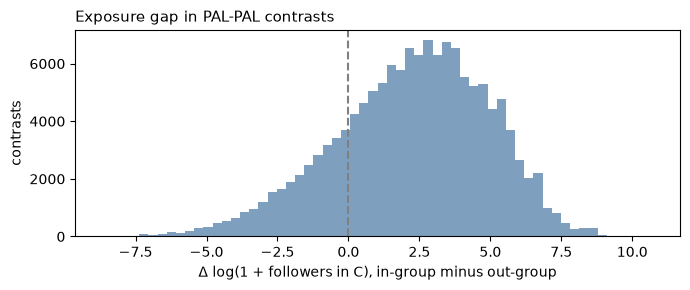
\includegraphics[width=0.85\textwidth]{figures/exposure_gap.png}
\caption{Exposure gap in PAL--PAL contrasts: $\Delta_r \log(1 + F^{C})$, the in-group author's
followers in $C$ minus the out-group author's, on a log scale.}
\label{fig:exposure-gap}
\end{figure}

\subsection{Confirmatory results}\label{sec:confirmatory}

Apropos of our primary outcome, we find no detectable in-group advantage for pro-Palestinian pairings as 1 lies within the confidence interval of every tested measure (see Table~\ref{tab:primary-outcomes}). 
It should be noted that the observed interval is narrow enough to itself be informative:
at equal exposure, it is consistent with the in-group post receiving between about 47\% and 56\% of
the pair's reposts from $C$, and rules out an in-group advantage larger than roughly 27\%. Additionally, we can observe that all of our robustness
checks confirm this result (see Table~\ref{tab:robustness}).

\begin{table}[h]
\centering
\begin{tabular}{lrcc}
\toprule
Outcome & Contrasts & RR (95\% CI) & $p$ \\
\midrule
\textbf{Reposts (primary)} & 138,060 & \textbf{1.05} (0.87--1.27) & 0.59 \\
Replies                    & 90,333  & 1.07 (0.92-1.24) & 0.40 \\
Quotes                     & 25,961  & 1.27 (0.90-1.80) & 0.18 \\
Negative-tone replies      & 62,956  & 1.06 (0.89-1.27) & 0.52 \\
\bottomrule
\end{tabular}
\caption{In-group rate ratios for PAL--PAL contrasts in the primary sample.}
\label{tab:primary-outcomes}
\end{table}

\begin{table}[h]
\centering
\begin{tabular}{lrc}
\toprule
Specification (reposts) & Contrasts & RR (95\% CI) \\
\midrule
Primary                                   & 138,060 & 1.05 (0.87-1.27) \\
Exposure-matched                          & 24,642  & 1.04 (0.83-1.30) \\
Both labels confidence $\geq 2$           & 133,725 & 1.05 (0.87-1.27) \\
Drop short, near-duplicate, linked pairs  & 114,407 & 1.10 (0.91-1.34) \\
Similarity $\geq 0.85$                    & 41,827  & 1.01 (0.76-1.35) \\
At most 5 contrasts per post$^{\dagger}$  & 47,541  & 1.04 (0.86-1.25) \\
\midrule
PAL-ISR (opposite sides, comparison)     & 19,408  & 0.77 (0.45--1.34) \\
\bottomrule
\end{tabular}
\caption{Robustness of the primary estimate. $^{\dagger}$Cap chosen after the primary model was run.}
\label{tab:robustness}
\end{table}

In terms of communities, 4 and 1, which together contribute most of the primary sample (63,213 and 44,641
contrasts), both yield confidence intervals including 1 (0.95-1.52 and 0.84-1.70 respectively). In contrast, community 6 is
the sole large community with a demonstrable in-group effect: RR is 2.78 with an interval of 1.95 to 3.96 (see Figure~\ref{fig:community-forest}).

\begin{figure}[h]
\centering
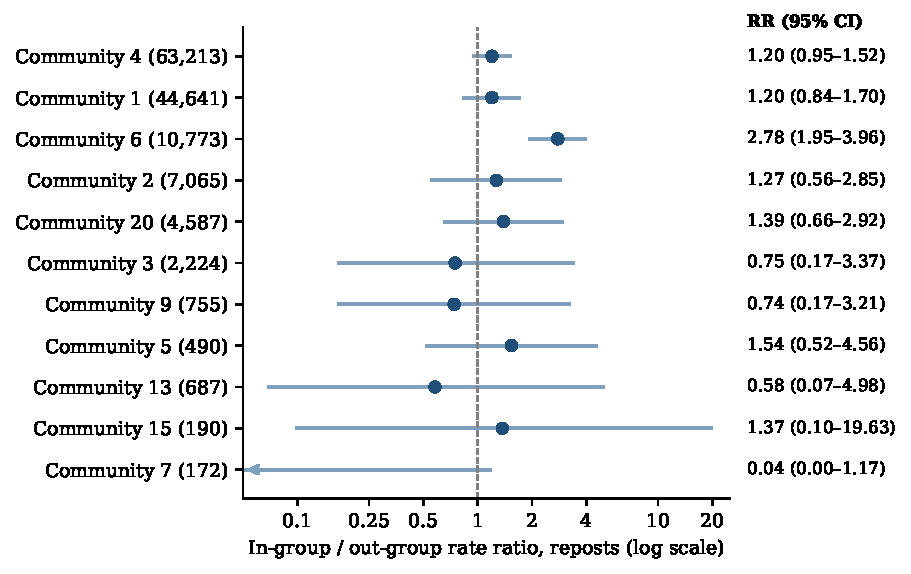
\includegraphics[width=0.9\textwidth]{figures/community_forest.pdf}
\caption{In-group rate ratios for reposts in PAL-PAL contrasts by community with 95\% confidence
intervals. The bracketed numbers to the left are contrasts with at least one repost from $C$. Communities 40, 14, 19
and 8 are omitted due to the size of their confidence intervals; community 7's estimate (0.04) lies
off the left of the axis.}
\label{fig:community-forest}
\end{figure}

\subsection{Exploratory results}\label{sec:exploratory}

\subsection*{Pro-Israeli pairs}
Unlike our primary outcome, the exploratory ISR-ISR contrasts do show an in-group advantage in reposts, with $\text{RR}=1.73$ (CI: 1.05-2.86, $p = 0.03$), with similar
estimates for replies (1.52) and negative-tone replies (1.69). This can't just be attributed to label noise since in a follow-up hand annotated set of 50 random ISR-ISR pairs by the author, 
we found that both posts were truly pro-Israeli 94\% of the time (95\% CI 84-98\%) and falsely pro-Palestinian never. The estimate points the same way in every large community, and dropping
any single community leaves it between 1.58 and 2.06 with a still non-null result. Still, this measure is nonetheless fragile and remains exploratory. It is one of roughly
40 estimates reported, it rests on 4,968 contrasts, and dropping the five most-reposted in-group
authors reduces it to 1.43 with a CI containing 1 (0.92-2.22).

\subsection*{Community 6}
Community 6 appears to revolve around British and Irish politics, and carries the most neutral news of the large communities. Its pro-Palestinian in-group effect
is hardy, surviving exposure matching (3.10), the dropping of its ten most-reposted in-group authors (2.38)
or its ten heaviest reposters (2.69), the exclusion of posts that mention the UK (2.79), and the restricting to
pairs posted within two hours of each other (2.66). This case was identified post hoc.

\subsection{Limitations}\label{sec:limitations}
\begin{itemize}
    \item Likes are not analysed as the data carries no liker identifiers.
    \item Due to financial limitations no stronger model was used, a more well-equipped study would be capable of much more precise stance labelling.
    \item Similar to the above point only a set of 200 posts was labelled for development and only another 198 for testing, each done by a solo coder.
    To make the $\kappa$ value more interpretable and improve accuracy (especially for the rarer stances like pro-Israeli), a more well-staffed study could
    provide a more trustworthy set of estimates.
    \item Positive and negative engagement could be very well gauged by the labelling of replies themselves, again precluded in this instance by financial considerations. The negative tone replies we use as a secondary measure was included in the dataset, but does not track stance.
    \item This method addresses same stance communities, not cross-cutting views themselves. This was done in the interest of time, but a better reply to the questions raised in the introduction would be extending this to cross stance analysis. 
\end{itemize}

\section{Conclusion}\label{sec:conclusion}
Ultimately, no substantial evidence could be found for a hell of the Same in the network of Bluesky qua the Israeli-Palestinian split.
In fact, in-group authors appear to have surprisingly little advantage controlling for exposure effects, at least for the pro-Palestinian communities that dominate the platform. This by no means rejects the broad notion of a hell of the Same as the theory is unfalsifiable,
but in this specific instance we find evidence to the contrary of our particular formulation. Of course, we studied the an environment saturated overwhelmingly with one stance,
so its possible that there is not Other left to consume, the hell of the Same could operate on the level of platform (X vs Bluesky) instead, but further study would be required. \bigskip

In terms of concrete policy, since exposure seemed to account for the vast majority of what people encounter, platforms and
policymakers should focus on feed tailoring and follow recommendations rather than users' attitudes towards out-group
authors. Also, auditors looking at raw engagement shares would have concluded that there is strong in-group favoritism,
but our analysis demonstrates the opposite once weighted. We would recommend audits adjust for audience size as well
as per community, since community 6 showed disparate results from the rest as did ISR-ISR pairings more broadly. Our results would offer tenuous support for bridging
between communities being a valid strategy, but would again advise on evaluation via a community by community basis.\bigskip

\section{AI Appendix}
Claude Opus 5.5 was used extensively for the coding implementation of this project, mostly in the interest of time. Certain aspects of the code,
like data exploration and graph construction, were done by hand, but I quickly realized that setting up a full labelling pipeline is unfeasible in a weekend.
I don't have any logs to provide since these are all local conversations on my machine, but one such prompt were pretty much just "draft a pipeline to evaluate same-content pairs using FAISS."
Claude was similarily used for table and graph representations on the final paper, but writing, problem formulation, and research were all owned by me; additionally 
all of the code written by the AI was reviewed and in certain cases cleaned up or annotated by hand. \bigskip

\noindent Link to the GH Repo: https://github.com/pasupasu/bluesky-case-study.git

\printbibliography 
\end{document}